\section{Introduction}
Defined the marXbot \cite{bonani2010marxbot} as the target platform, whose main 
characteristic is a rotating laser scanner, which perceives distances and 
colours of objects surrounding the robot. The experiments are run in Enki  
\cite{enki}, a high-performance open-source simulator for planar robots. Enki 
provides collision and limited physics support for robots evolving on a flat 
surface. 
Moreover, it can simulate groups of robots hundreds of times faster than real-time.

\begin{figure}[htbp]
	\centerline{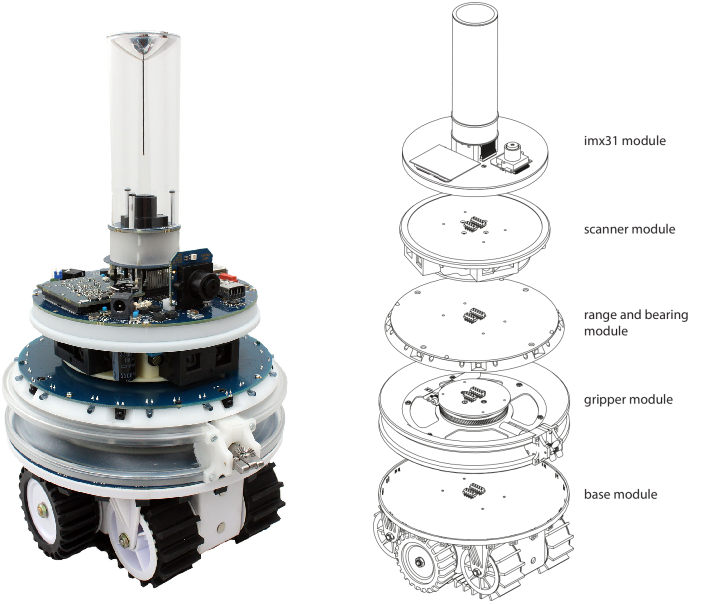
\includegraphics[width=.8\columnwidth]{introduction/marxbot}}
	\caption{Actual image and exploded CAD view of a marXbot.}
	\label{fig:marxbot}
\end{figure}

The main objective of this project is learning to perform specific interactions between the robot and objects in the 
environment.
Write an omniscient controller that performs the desired interaction with complete knowledge of the environment (e.g. 
position the robot at a certain location relative to an object) using Enki.
Generate a dataset of simulation runs through Enki. 
Through imitation learning, train an end-to-end neural network that receives as inputs the sensor distances and the 
camera image readings and produces commands for the motors that are the left and the right wheel target speeds.
Evaluate the model trained using Enki.
See \cite{pitch} for a brief pitch of the project. FIXME add final video
